\documentclass[12pt,a4paper]{article}
\usepackage[utf8]{inputenc}
\usepackage{amsmath}
\usepackage{amsfonts}
\usepackage{amssymb}

\usepackage{cmap} % для кодировки шрифтов в pdf
\usepackage[T1]{fontenc}
\usepackage{hhline}
\usepackage[unicode]{hyperref}
\usepackage{multirow}
\usepackage{array}
\usepackage{amsmath}
\usepackage{bm}
\usepackage{textcomp}
\usepackage[russian]{babel}
\usepackage{graphicx} % для вставки картинок
\usepackage{amssymb,amsfonts,amsmath,amsthm} % математические дополнения от АМС
\usepackage{indentfirst} % отделять первую строку раздела абзацным отступом тоже
% Поля
\usepackage{geometry}
\geometry{left=2cm}
\geometry{right=1.5cm}
\geometry{top=2.4cm}
\geometry{bottom=2.cm}

%%%%%%%%%%%%%%%%%%%%%%%%%%%%%%%     

\linespread{1.5} % полуторный интервал
\frenchspacing

\begin{document}
	
	\begin{titlepage}
		
		\begin{center}
			\begin{large}
				Санкт-Петербургский Политехнический университет\\ Петра Великого\\
				Институт прикладной математики и механики\\
			\end{large}
			\vspace{0.2cm}
			Высшая школа прикладной математики и вычислительной физики\\
			
		\end{center}
		
		\vspace{3cm}
		\begin{center}
			\textbf{Отчёт\\ по лабораторной работе 6\\ по дисциплине\\ "математическая статистика"}
		\end{center}
		
		\vspace{3cm}
		\vbox{%
			\hfill%
			\vbox{%0
				\hbox{Выполнил студент:}%
				\hbox{\break}
				\hbox{Аникин Александр Алексеевич,}%
				\hbox{группа 3630102$\backslash$80201}%
				\hbox{\break}
				\hbox{\break}
				\hbox{Проверил:}
				\hbox{\break}
				\hbox{к.ф.-м.н., доцент}
				\hbox{Баженов Александр Николаевич}
			}%
		} 
		\vfill
		
		\begin{center}
			Санкт-Петербург\\2021
		\end{center}
		
	\end{titlepage}
	\tableofcontents
	\newpage
	
	\listoffigures
	\newpage
	
	\section{Постановка задачи}
		Найти оценки коэффициентов линейной регрессии $y_i=a+bx_i+e_i$ используя 20 точек на отрезке $[-1.8; 2]$ с равномерным шагом равным
		$0.2$. Ошибку $e_i$ считать нормально распределённой с параметрами $(0,
		1)$. В качестве эталонной зависимости взять $y_i = 2 + 2x_i$. При построении оценок коэффициентов использовать два критерия: критерий наименьших квадратов и критерий наименьших модулей. Проделать то же самое для выборки, у которой в значения $y_1$ и $y_{20}$ вносятся
		возмущения $10$ и $-10$.
	\newpage
	
	\section{Теория}
		\subsection{Модель простой линейной регрессии}
			Регрессионную модель описания данных называют простой линейной регрессией, если
			\begin{equation}
				y_i = \beta_0+\beta_1 x_i + \epsilon_i
			\end{equation} 
			где $x_1, ... , x_n$ — заданные числа (значения фактора); $y_1, ... , y_n$ — наблюдаемые значения отклика; $\epsilon_1, ... , \epsilon_n$ — независимые, нормально распределённые $N(0, \sigma)$ с нулевым математическим ожиданием и одинаковой (неизвестной) дисперсией случайные величины; $\beta_0, \beta_1$ —
			неизвестные параметры, подлежащие оценке.
		\subsection{Метод наименьших квадратов}
			Метод наименьших квадратов (МНК):
			\begin{equation}
				Q(\beta_0,\beta_1)=\sum_{i=1}^{n}\epsilon_i^2=\sum_{i=1}^{n}(y_i-\beta_0-\beta_1 x_i)^2 \rightarrow \underset{\beta_0, \beta_1}\min	
			\end{equation}
			Расчётные формулы для МНК оценок:
			\begin{equation}
				\hat{\beta_1}=\frac{\overline{xy}-{\overline{x}}* {\overline{y}}}{\overline{x^2}-{\overline{x}}^2}
			\end{equation}
			\begin{equation}
				\hat{\beta_0}=\overline{y}-\overline{x}\hat{\beta_1}
			\end{equation}
		\subsection{Метод наименьших модулей}
			Метод наименьших модулей(МНМ):
			\begin{equation}
				\sum_{i=1}^{n}|y_i-\beta_0-\beta_1 x_i|\rightarrow\underset{\beta_0, \beta_1}\min	
			\end{equation}
			Расчётные формулы для МНМ оценок:
			\begin{equation}
				r_Q=\frac{1}{n}\sum_{i=1}^{n}sgn(x_i-med(x))sgn(y_i-med(y))
			\end{equation}
			
			\begin{equation}
				q_y^*=\frac{y_j-y_l}{k_q(n)}, \quad q_x^*=\frac{x_j-x_l}{k_q(n)},
			\end{equation}
		
			\begin{equation}
				l = 
				\left\{
				\begin{array}{l}
					\frac{n}{4} + 1 \quad \text{при} \quad \frac{n}{4} \quad \text{дробном}\\
					\quad \frac{n}{4} \qquad \text{при} \quad \frac{n}{4} \quad \text{ целом}
				\end{array}
				\right.
				, \quad j = n - l + 1
			\end{equation}

			
			\begin{equation}
				\hat{\beta_1}=r_Q\frac{q_y^*}{q_x^*}
			\end{equation}
			\begin{equation}
				\hat{\beta_0}=med(y)-\hat{\beta_1}med(x)
			\end{equation}
	\newpage
	
	\section{Реализация}
	Лабораторная работа выполнена на языке Python 3.8 с помощью загружаемых пакетов SciPy, MatPlotLib, NumPy. Исходный код лабораторной работы находится на GitHub репозитории.
	\newpage
	
	\section{Результаты}
		\subsection{Оценка коэффициентов линейной регрессии}
			\subsubsection{Выборка без возмущений}
				\begin{itemize}
					\item Метод наименьших квадратов:
					\begin{center}
						$a \approx 2.08, \quad b \approx 1.85$
					\end{center}
					\item Метод наименьших модулей:
					\begin{center}
						$a \approx 1.55, \quad b=1.03$
					\end{center}
				\end{itemize}
				\begin{figure}[h!]
					{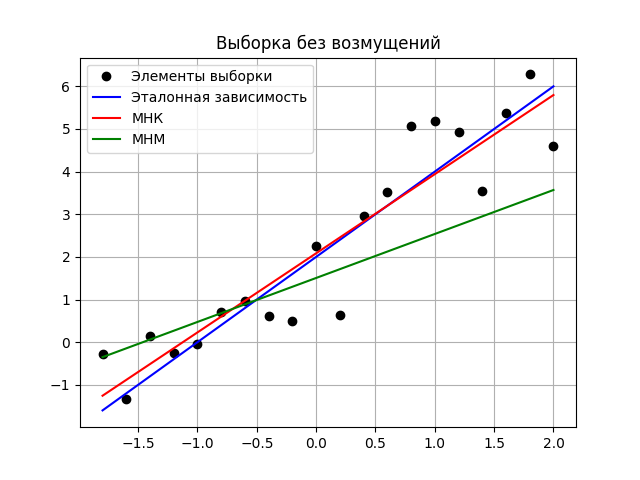
\includegraphics[width=1\linewidth]{../plots/default.png}}
					\caption{Выборка без возмущений}
				\end{figure}
			\clearpage
			
			\subsubsection{Выборка с возмущениями}
				\begin{itemize}
					\item Метод наименьших квадратов:
					\begin{center}
						$a \approx 2.22, \quad b \approx 0.42$
					\end{center}
					\item Метод наименьших модулей:
					\begin{center}
						$a \approx 1.56, \quad b=1.77$
					\end{center}
				\end{itemize}
				\begin{figure}[h!]
					{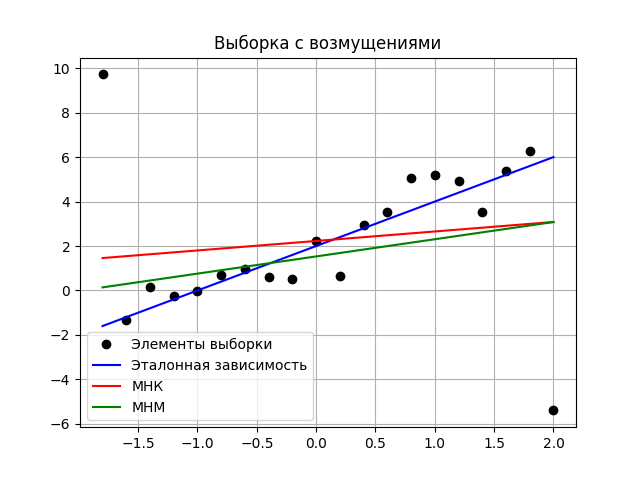
\includegraphics[width=1\linewidth]{../plots/altered.png}}
					\caption{Выборка с возмущениями}
				\end{figure}
			\clearpage
			\section{Обсуждение}
			Стоит заметить, что в случае выборки без значительных возмущений метод наименьших квадратов дает более точную оценку чем метод наименьших модулей, однако при внесении возмущений в краевые точки выборки МНК показывает довольно сильное отклонение, МНМ остается относительно близок к эталонной модели (ближе чем МНК). На основании проведенного исследования можно установить, что при малых отклонениях исходных данных целесообразнее использовать метод наименьших квадратов, в противном случае - метод наименьших модулей.
			\newpage
\end{document}